\chapter{Work Methodology} \label{chapter_four}

We will be using an IMU sensor for camera pose estimation to stabilize the video for this work. Based on the precision requirements of the pose-estimation algorithm we will be using a data-driven approach as classical signal processing and sensor fusion algorithms fail to provide this precision over a long period of time. For our data driven approach we build datasets using a camera and also simulation. To capture the video we are using a GoPro Hero 10 which provides synchronised image and sensor data capture. We also swapped the factory lens to a low Field of View (FOV) and high focal length lens. The simulation was build using Unreal Engine 4 and Microsoft AirSim. Table \ref{tab:technical_details} shows the technical specifications of the camera setup. For simulation similar camera parameters were used.

\begin{table}
    \centering
\begin{tabular}{ c| c | L }

     Image Sensor & 
     Sony & 
     Diagonal 7.85 mm (Type 1/2.3) 23.91 M CMOS Image Sensor with Square Pixel. \\
     \hline
     
     IMU Sensor & 
     Bosch & 
     6-axis IMU Sensor
     Accelerometer (A): 16-bit or 0.06 mg/LSB 
     Gyroscope (G): 16-bit or 0.004 dps/LSB  \\
     \hline
     
     Lens & 
     xx & 
     15° FOV and 00 mm focal length \\

\end{tabular}
    \caption{Technical Specification}
    \label{tab:technical_details}
\end{table}

\section{Data Collection}
Collecting data for any data driven approach is a challenging and an iterative process. The data or training data in this case are the readings coming from the IMU sensor and the target (ground truth) being the camera pose (position and orientation). Real data was collected by mounting the camera on a rig which had vibrations associated with it on movement. We made sure that the data depicts real life scenarios by moving the rig around in many different ways and let it vibrate and collect the data. The ground truth was generated using proprietary Zeiss software and is beyond the scope of this work. 

Then the data was collected from simulation based on the analysed real data and pushed beyond real data limits to account for even more challenging scenarios. Generating simulated data with accurate ground truth is a fast processes not requiring much post-processing. This also allowed us to tinker with noise and bias to make the neural network robust and generalize well.

\subsection{Data Analysis}
\label{data_analysis}
The data recorded from a camera-rig setup was analysed to determine the vibration and sensor parameters. Table \ref{tab:imu_noise_characteristics} summarises the white noise and bias characteristics determined from the raw IMU Sensor Readings. These match closely with the data provided by the manufacturer. Accelerometer variance from data sheet $ 160 \mu g /\sqrt{Hz} $ and for gyroscope $ 0.008 dps /\sqrt{Hz}  $.

\begin{table}[ht]
\centering
\begin{tabular}{l|c}
    Parameter & Value \\ \hline
    Accelerometer Bias & xx \\  
    Accelerometer White Noise & $ \mu = 0 $ and $ \sigma^{2}=0.xxx $ \\  
    Gyro Bias & xx \\  
    Gyro White Noise & $ \mu = 0 $ and $ \sigma^{2}=0.xxx $ \\  
\end{tabular}
\caption{IMU Noise Characteristics}
\label{tab:imu_noise_characteristics}
\end{table}

We analysed the generated ground truth to determine the characteristics of vibration. These characteristics are important to understand the nature of vibration and to set the working limits for our work. Vibrations are characterised by \textbf{Amplitude} ( A or  $ \theta $), \textbf{Time Constant} ($ \tau $) and \textbf{Frequency} ($ \omega $). We have damped oscillations for both displacement and rotation vibration as shown in figure \ref{fig:damped_vib} and can be characterised by the equations \ref{eqn:vib_disp} and \ref{eqn:vib_rot}.

\begin{figure}
    \centering
    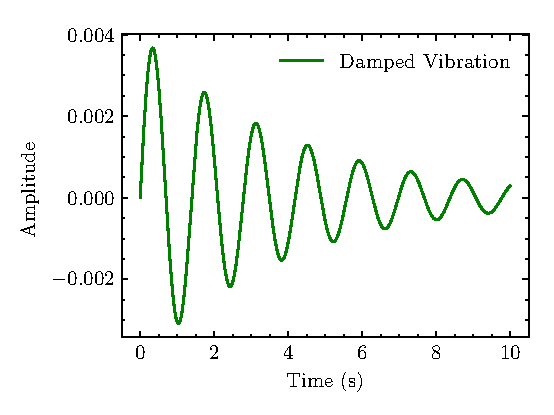
\includegraphics{images/fig_chapter4/vib_damped.eps}
    \caption{Damped Vibration}
    \label{fig:damped_vib}
\end{figure}

\begin{equation}
  \label{eqn:vib_disp}
  \begin{aligned}
    A(t) = Ae^{-t/\tau}sin(2\pi\omega t) \\
  \end{aligned}
\end{equation}

\begin{equation}
  \label{eqn:vib_rot}
  \begin{aligned}
    \theta(t) = \theta e^{-t/\tau}sin(2\pi\omega t) \\
  \end{aligned}
\end{equation}

%% Displacement distribution
\begin{figure}
    %%
    \begin{subfigure}{\linewidth}
    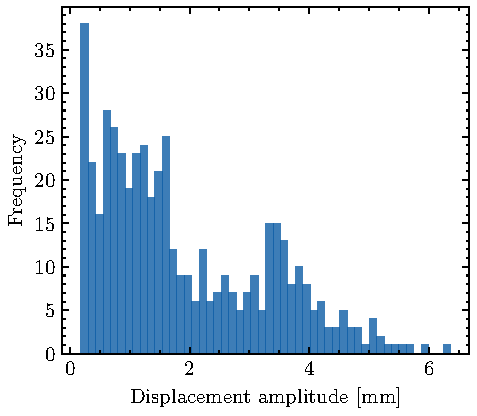
\includegraphics[width=.5\linewidth]{images/fig_chapter4/data_dist/1.pdf}\hfill
    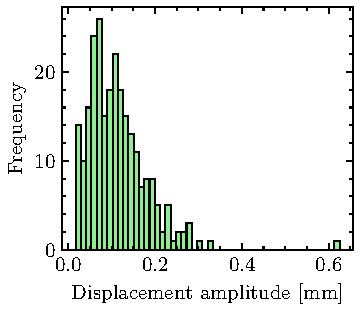
\includegraphics[width=.5\linewidth]{images/fig_chapter4/data_dist/2.pdf}
    \caption{Distribution of displacement amplitude $ A $ in XY(left) and Z(right) DoF [mm]}
    \end{subfigure}\par\medskip
    
    %%
    \begin{subfigure}{\linewidth}
    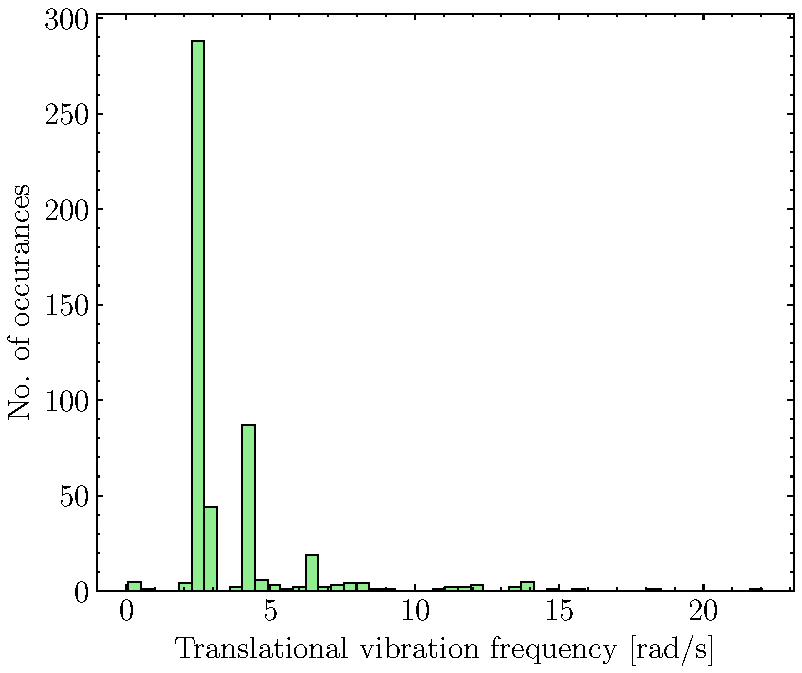
\includegraphics[width=.5\linewidth]{images/fig_chapter4/data_dist/3.pdf}\hfill
    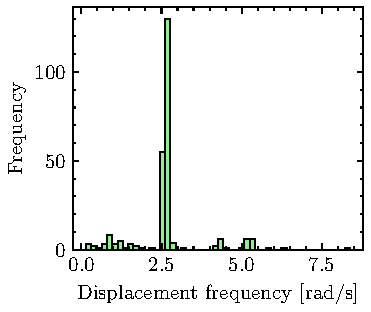
\includegraphics[width=.5\linewidth]{images/fig_chapter4/data_dist/4.pdf}
    \caption{Distribution of displacement frequency $ \omega $ in XY(left) and Z(right) DoF [mm]}
    \end{subfigure}\par\medskip
    
    %%
    \begin{subfigure}{\linewidth}
    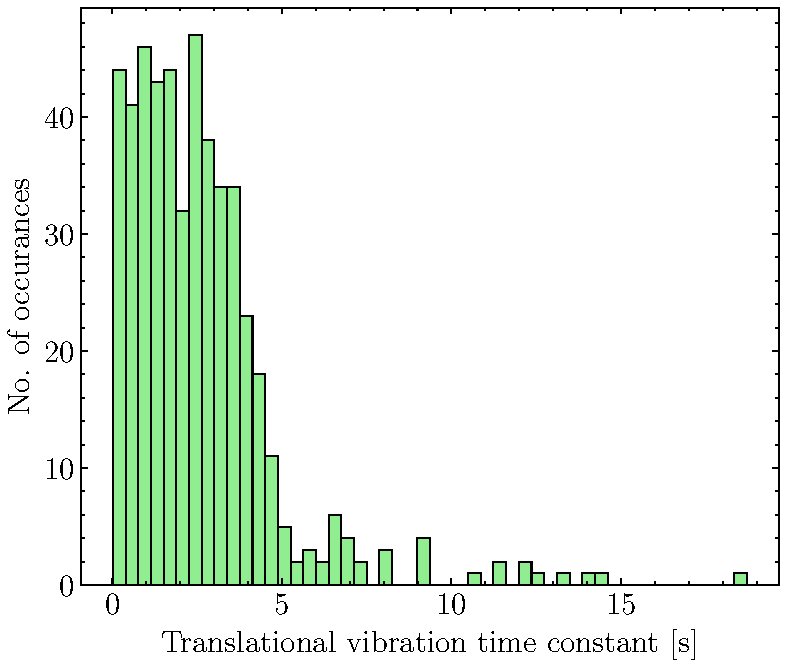
\includegraphics[width=.5\linewidth]{images/fig_chapter4/data_dist/5.pdf}\hfill
    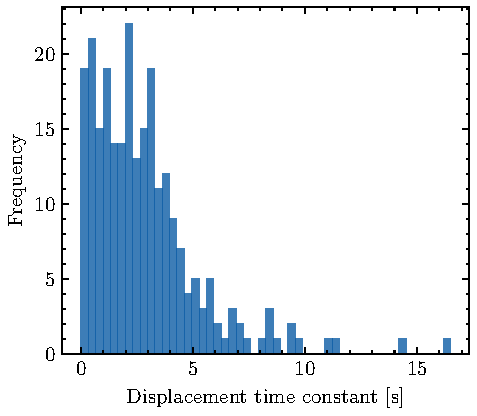
\includegraphics[width=.5\linewidth]{images/fig_chapter4/data_dist/6.pdf}
    \caption{Distribution of displacement time-constant $ \tau $ in XY(left) and Z(right) DoF [mm]}
    \end{subfigure}
\caption{Real displacement data statistical analysis}
\label{fig:dist_disp}
\end{figure}

%% Rotation Distribution 
\begin{figure}
    %%
    \begin{subfigure}{\linewidth}
    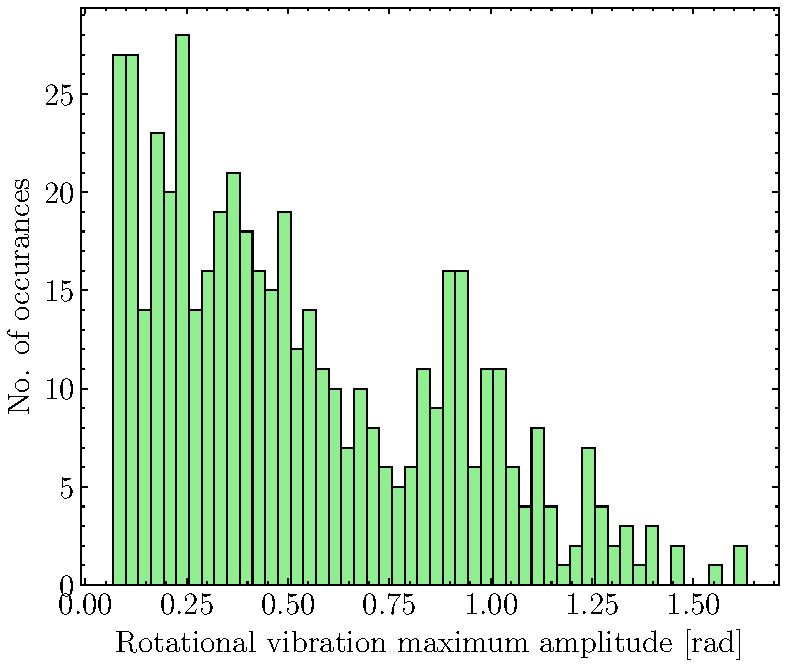
\includegraphics[width=.5\linewidth]{images/fig_chapter4/data_dist/7.pdf}\hfill
    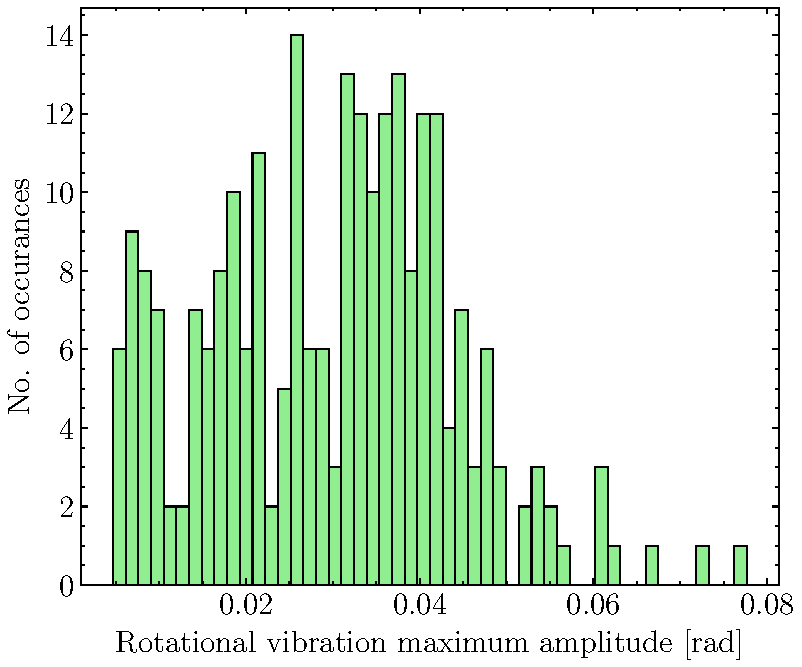
\includegraphics[width=.5\linewidth]{images/fig_chapter4/data_dist/8.pdf}
    \caption{Distribution of rotation amplitude $ \theta $ in XY(left) and Z(right) DoF [mm]}
    \end{subfigure}\par\medskip
    
    %%
    \begin{subfigure}{\linewidth}
    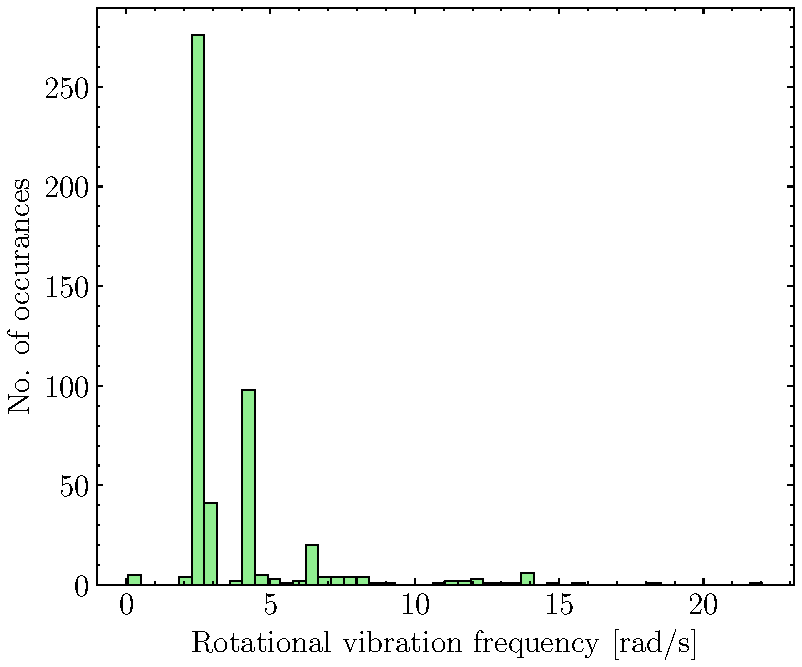
\includegraphics[width=.5\linewidth]{images/fig_chapter4/data_dist/9.pdf}\hfill
    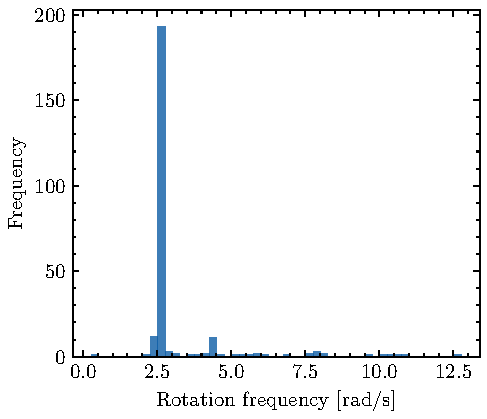
\includegraphics[width=.5\linewidth]{images/fig_chapter4/data_dist/10.pdf}
    \caption{Distribution of rotation frequency $ \omega $ in XY(left) and Z(right) DoF [mm]}
    \end{subfigure}\par\medskip
    
    %%
    \begin{subfigure}{\linewidth}
    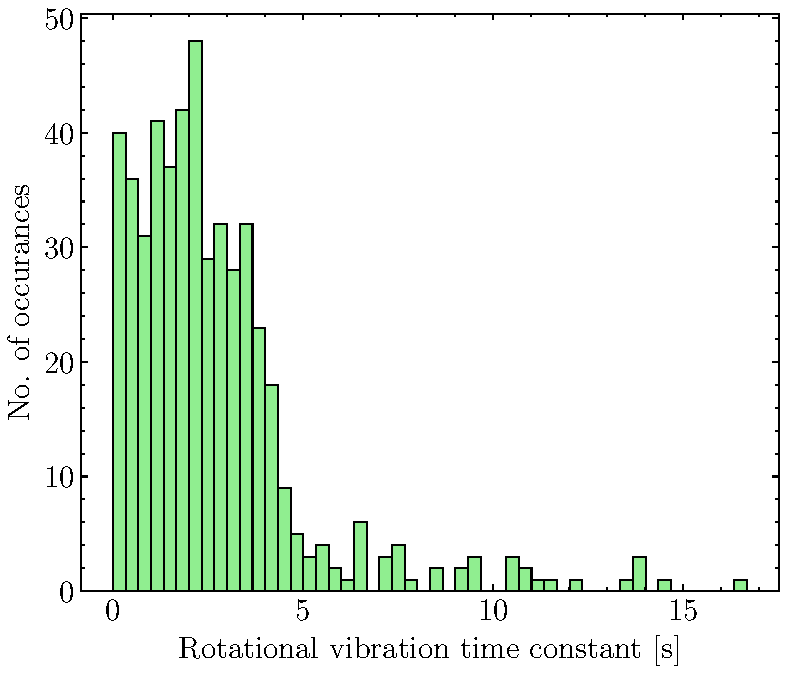
\includegraphics[width=.5\linewidth]{images/fig_chapter4/data_dist/11.pdf}\hfill
    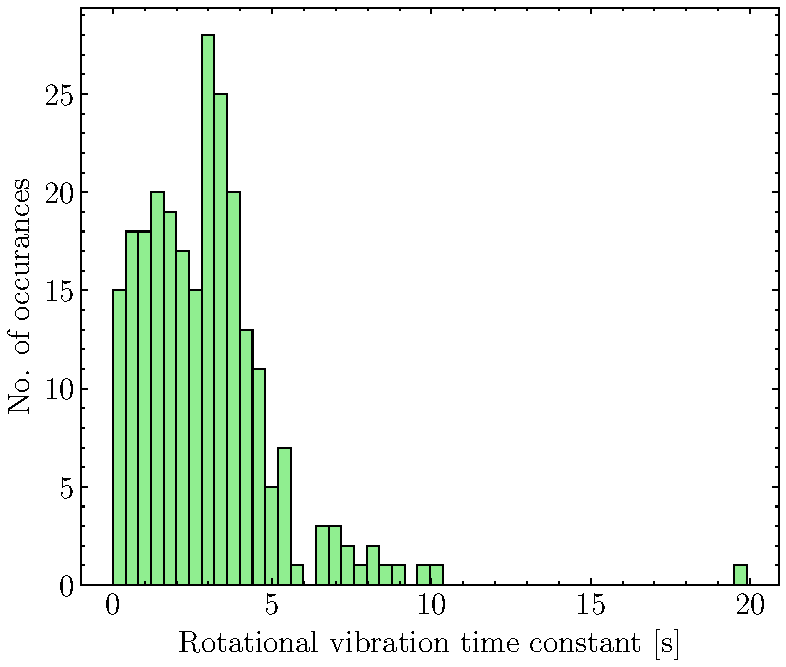
\includegraphics[width=.5\linewidth]{images/fig_chapter4/data_dist/12.pdf}
    \caption{Distribution of rotation time-constant $ \tau $ in XY(left) and Z(right) DoF [mm]}
    \end{subfigure}

\caption{Real rotation data statistical analysis}
\label{fig:dist_rot}
\end{figure}


The statistical analysis shown in figure \ref{fig:dist_disp} and figure \ref{fig:dist_rot} was done on 248 vibration sequences with an average length of 10 seconds. The results for displacement and rotation vibrations are summarised in table \ref{tab:real_data_analysis_displacement} and table \ref{tab:real_data_analysis_rotation} respectively. The rotational vibrations have very small amplitude ($ \theta $) and is less than 1 degrees for more than 75 percent of the samples in XY plane. For Z axis the vibrations are even smaller with a mean of 0.0005 degrees. These vibrations are very small and do not have a a noticeable visual effect on the video stabilization. But we have decided to account for them to develop a more general solution with multiple applications. The time constant ($ \tau $) for displacement and rotation is similar for all DoF with a mean value of around 2.9 seconds.  The frequency ($ \omega $) for all DoF is also similar in the range $ 2.5 rad/sec $ to $ 3.5 rad/sec $. Frequency of $ 2.5 rad/sec $ is the most dominant frequency and seems to be the natural frequency $ \omega_n $ of the mechanical system (rig on which the camera is mounted).


The amplitude ($ A $) of the vibration displacement is the most important characteristic for this work as it is main source of video destabilization. The effect of motion on the quality of video is more pronounced in XY plane as the most pixel shift happens here. In Z axis the mean ($ \mu $) of vibrations is 0.113 mm with a standard deviation ($ \sigma^{2} $) of 0.07 mm. Even the large vibrations in Z seem to have little effect on visual quality of the video. Vibrations in XY plane have the mean of 1.9 mm with a standard deviation of 1.36 mm. Vibrations with higher magnitude are also present and need to be accounted for when generating simulated data.




% displacement data distribution table
\begin{table}[ht]
    \centering
\begin{tabular}{ c | L | L | L }
    
     Parameter  & 
     Mean ($ \mu $) & 
     Variance ($ \sigma^{2} $) &
     Standard Deviation ($ \sigma $)\\
     \hline
     
     $ A_{xy} $ & 
     $ 1.8944 mm $ & 
     $ 1.8674 mm^{2} $ &
     $ 1.3665 mm $ \\

      
     $ A_{z} $  & 
     $ 0.1135 mm $ & 
     $ 0.0047 mm^{2} $ &
     $ 0.0690 mm $ \\
     
     
     $ \omega_{xy} $ & 
     $ 3.6898 rad/s $ & 
     $ 5.9833 rad^{2}/s^{2} $ &
     $ 2.4460 rad/s $ \\
     
     
     $ \omega_{z} $& 
     $ 2.6835 rad/s $ & 
     $ 2.0765 rad^{2}/s^{2} $ &
     $ 1.0375 rad/s $ \\

     
     $ \tau_{xy} $ & 
     $ 2.5914 s $ & 
     $ 5.1898 s^{2} $ &
     $ 2.2781 s $ \\


     $ \tau_{z} $ & 
     $ 2.8396 s $ & 
     $ 5.8720 s^{2} $ &
     $ 2.4243 s $ \\

\end{tabular}
    \caption{Real Data displacement-vibration distributions}
    \label{tab:real_data_analysis_displacement}
\end{table}

% rotation data distribution table
\begin{table}[ht]
    \centering
\begin{tabular}{ c | L | L | L }

     Parameter  & 
     Mean ($ \mu $) & 
     Variance ($ \sigma^{2} $) &
     Standard Deviation ($ \sigma $)\\
     \hline
     
     $ \theta_{xy} $ & 
     $ 0.0094 rad $ & 
     $ 3.8729e^{-8} rad^{2} $ &
     $ 0.0062 rad $ \\

      
     $ \theta_{z} $  & 
     $ 0.0005 rad $ & 
     $ 6.0739e^{-8} rad^{2} $ &
     $ 0.0002 rad $ \\
     
     
     $ \omega_{xy} $ & 
     $ 3.8042 rad/s $ & 
     $ 6.3685 rad^{2}/s^{2} $ &
     $ 2.5236 rad/s $ \\

     
     $ \omega_{z} $& 
     $ 3.1763 rad/s $ & 
     $ 2.6238 rad^{2}/s^{2} $ &
     $ 1.6198 rad/s $ \\
   
     
     $ \tau_{xy} $ & 
     $ 2.6581 s $ & 
     $ 5.8362 s^{2} $ &
     $ 2.4158 s $ \\
    
     
     $ \tau_{z} $ & 
     $ 2.9316 s $ & 
     $ 4.7336 s^{2} $ &
     $ 2.1757 s $ \\

\end{tabular}
    \caption{Real Data rotational-vibration distributions}
    \label{tab:real_data_analysis_rotation}
\end{table}



\subsection{Simulated Data Generation}
\label{sec:gen_sim_data}
The simulated data plays a very important role in our approach as we use the ideal data to validate our stabilization approach. It also empowers us to simulate IMU sensors with different noise levels and characteristics. We also made sure that the data generated from the simulation is fairly domain randomized to make it realistic. 

Simulated data is based on the analysed real data with vibration characteristics taken from table \ref{tab:real_data_analysis_displacement} and table \ref{tab:real_data_analysis_rotation}. The data is then generated using the equations \ref{eqn:vib_disp} and \ref{eqn:vib_rot} .The simulated data is then augmented with modified noise and bias characteristics from table \ref{tab:imu_noise_characteristics}. A total of 600 vibration sequences with an average vibration duration of 15 seconds was generated with characteristics shown in tables \ref{tab:real_data_analysis_displacement} and \ref{tab:real_data_analysis_rotation}. Generating a large number of samples ensures the sampling of diverse data from the distribution. This is where we benefit from our simulation the most as the diversity and the size of data ensures our neural network generalizes well.



% Sim Vibration characteristics
 \begin{table}[ht]
\centering
\begin{tabular}{ c | L | L | L }
    
     Parameter  & 
     Mean ($ \mu $) & 
     Variance ($ \sigma^{2} $) &
     Standard Deviation ($ \sigma $)\\
     \hline
     
     $ A_{xy} $ & 
     $ 2.5 mm $ & 
     $ 2.2 mm^{2} $ &
     $ 1.48 mm $ \\

      
     $ A_{z} $  & 
     $ 0.4 mm $ & 
     $ 0.01 mm^{2} $ &
     $ 0.1 mm $ \\
     
     
     $ \omega_{xy} $ & 
     $ 4.5 rad/s $ & 
     $ 6.5 rad^{2}/s^{2} $ &
     $ 2.55 rad/s $ \\
     
     
     $ \omega_{z} $& 
     $ 3.5 rad/s $ & 
     $ 2.5 rad^{2}/s^{2} $ &
     $ 1.58 rad/s $ \\

     
     $ \tau_{xy} $ & 
     $ 3.5 s $ & 
     $ 6.0 s^{2} $ &
     $ 2.45 s $ \\


     $ \tau_{z} $ & 
     $ 3.5 s $ & 
     $ 6.0 s^{2} $ &
     $ 2.45 s $ \\
    
    \hline
    \hline
    
     $ \theta_{xy} $ & 
     $ 0.001 rad $ & 
     $ 5e^{-7} rad^{2} $ &
     $ 7.1^{-4} rad $ \\

      
     $ \theta_{z} $  & 
     $ 0.001 rad $ & 
     $ 6e^{-7} rad^{2} $ &
     $ 7.75^{-4} rad $ \\
     
     
     $ \omega_{xy} $ & 
     $ 4.5 rad/s $ & 
     $ 7 rad^{2}/s^{2} $ &
     $ 2.65 rad/s $ \\

     
     $ \omega_{z} $& 
     $ 4 rad/s $ & 
     $ 3 rad^{2}/s^{2} $ &
     $ 1.73 rad/s $ \\
   
     
     $ \tau_{xy} $ & 
     $ 3 s $ & 
     $ 6.2 s^{2} $ &
     $ 2.5 s $ \\
    
     
     $ \tau_{z} $ & 
     $ 3.3 s $ & 
     $ 5 s^{2} $ &
     $ 2.24 s $ \\
     
\end{tabular}
    \caption{Simulated vibration data characteristics}
    \label{tab:sim_vib_characteristics}
\end{table} %%%%


\section{Structuring of Data}
In classical pose-estimation techniques, every single IMU sample is used individually along with initial condition. Data driven approaches differ in this case as discussed in section \ref{sec:sota_pose_est}. For data driven approaches instead of taking an individual sample a \textit{window} of samples (figure \ref{fig:imu_window_samples})is used as a single sample does not contain enough information. Neural Networks unlike classical mathematics based approaches are data hungry and look for patterns in data and based on these patterns they generate an output. Initially we experimented with small window samples (3 - 20 samples) as shown in figure \ref{fig:imu_window_samples} a. This did not yield very good results and the pose estimation error was higher than the required. It started giving good results once we reach a IMU \textbf{ window size} of 70 to 140 samples (figure \ref{fig:imu_window_samples} b and c). Beyond these the performance does not improve much and the inferences from the neural network become computationally expensive and inference times become very high.

\begin{figure}
    \centering
    
\includegraphics{images/question_mark.eps}
    \caption{Different IMU window samples}
    \label{fig:imu_window_samples}
\end{figure}

\section{Mathematics for stabilisation}
Here we will see what exactly we are trying to find out: (R, T)

\section{Training and Testing of Various Neural Networks}
We will use various Neural Network types and Architectures.

\begin{itemize}
\item CNNs
\item RNNs: LSTMS 
\item Transformers
\item Temporal Fusion Transformers
\item CNNs
\item Resnets
\end{itemize}

\section{Image Stabilisation based on the Techniques Used}
We will see the Stabilized Videos and discuss about how they look visually to different people.


